\newpage 
\chapter{Тема 13 Файловые системы}

\begin{center}{\bfseries Файлы}
\end{center}
  

Файлы являются логическими информационными блоками, создаваемыми процессами. На диске обычно содержатся тысячи или даже миллионы не зависящих друг от друга файлов. Фактически если рассматривать каждый файл как некую разновидность адресного пространства, то это будет довольно близко к истине, за исключением того, что файлы используются для моделирования диска, а не оперативной памяти.

  \begin{center}{\bfseries Имена файлов}
  \end{center}

Файл является механизмом абстрагирования. Он предоставляет способ сохранения информации на диске и последующего ее считывания, который должен оградить пользователя от подробностей о способе и месте хранения информации и деталей фактической работы дисковых устройств. Наверное, наиболее важной характеристикой любого механизма абстрагирования является способ управления объектами и их именования, поэтому исследование файловой системы начнется с вопроса, касающегося имен файлов. Когда процесс создает файл, он присваивает ему имя. Когда процесс завершается, файл продолжает существовать, и к нему по этому имени могут обращаться другие процессы. Конкретные правила составления имен файлов варьируются от системы к системе, но все ныне существующие операционные системы в качестве допустимых имен файлов позволяют использовать от одной до восьми букв. Поэтому для имен файлов можно использовать слова andrea, bruce и cathy. Зачастую допускается также применение цифр и специальных символов, поэтому допустимы также такие имена, как 2, urgent! и Fig.2-14. Многие файловые системы поддерживают имена длиной до 255 символов.

\begin{center}{\bfseries Атрибуты файлов}
\end{center}
\begin{opr} 
  Атрибут файла — метаданные, которые описывают файл.
\end{opr}
Атрибут может находиться в двух состояниях: либо установленный, либо снятый. Атрибуты рассматриваются отдельно от других метаданных, таких как даты, расширения имени файла или права доступа. Каталоги и другие объекты файловой системы также могут иметь определённые атрибуты. Также существуют расширенные атрибуты файлов, хранящие данные другого типа.

\begin{center}{\bfseries Организация файлов}
\end{center}

\begin{opr} 
  Файл — это структура данных во внешней памяти, имеющая имя и специальную организацию.
\end{opr}

Во внешней памяти файлы только хранятся. Для обработки данные из файла вызываются в оперативную память. В каждый момент времени возможен доступ только к одному элементу файла. Этот элемент адресуется с помощью указателя файла.

\begin{center}{\bfseries Директории}
\end{center}

\begin{opr} 
  Директория — объект в файловой системе, упрощающий организацию файлов; позволяет сгруппировать файлы и, возможно, другие каталоги (для иерархических файловых систем).
\end{opr}

\begin{opr}
  Корневой каталог — каталог, прямо или косвенно включающий в себя все прочие каталоги и файлы файловой системы, называется корневым. 
\end{opr}
В Unix-подобных системах он обозначается символом /, в DOS и Windows исторически используется символ \, но с некоторого времени поддерживается и /. В DOS и Windows корневым считается каталог, который не является подкаталогом ни одного другого, это значит, каждый из томов в системе имеет свой корневой каталог (например, C:\, D:\ и так далее).

\begin{opr} 
  Текущий каталог — каталог, с которым работает система (оболочка или конкретная программа), если ей не указать другого каталога.
\end{opr}
В большинстве систем обозначается точкой. Для смены текущего каталога на другой используется в большинстве оболочек используется команда cd; без указания целевого каталога она меняет каталог на домашний (в Unix-подобных системах) или возвращает текущий (в Windows).

\begin{opr} 
  Родительский каталог — каталог, в котором находится текущий каталог, обозначается двумя точками (..), например, чтобы перейти в родительский каталог используется команда cd ...
\end{opr}
Обычно каталог реализуется как специальный файл, где регистрируется информация о других файлах и каталогах на носителе информации. Например, в Unix-системах — это файл, содержащий несколько inode и привязанные к ним имена. В современных Unix-подобных системах вводится структура каталогов, соответствующая стандарту FHS.

\begin{center}{\bfseries Структура файловой системы}
\end{center}

Файловые системы хранятся на дисках. Большинство дисков может быть разбито на один или несколько разделов, на каждом из которых будет независимая файловая система. Сектор 0 на диске называется главной загрузочной записью (Master Boot Record (MBR)) и используется для загрузки компьютера. В конце MBR содержится таблица разделов. Из этой таблицы берутся начальные и конечные адреса каждого раздела. Один из разделов в этой таблице помечается как активный. При загрузке компьютера BIOS (базовая система ввода-вывода) считывает и выполняет MBR. Первое, что делает программа MBR, — находит расположение активного раздела, считывает его первый блок, который называется загрузочным, и выполняет его. Программа в загрузочном блоке загружает операционную систему, содержащуюся в этом разделе. Для достижения единообразия каждый раздел начинается с загрузочного блока, даже если он не содержит загружаемой операционной системы. Кроме того, в будущем он может содержать какую-нибудь операционную систему.


\begin{center}{\bfseries Управление дисковым пространством}
\end{center}

Обычно файлы хранятся на диске, поэтому управление дисковым пространством является основной заботой разработчиков файловой системы. Для хранения файла размером n байт возможно использование двух стратегий: выделение на диске n последовательных байтов или разбиение файла на несколько непрерывных блоков. Такая же дилемма между чистой сегментацией и страничной организацией присутствует и в системах управления памятью.

\begin{center}{\bfseries Учёт свободного места}
\end{center}

Дисковое пространство, не выделенное ни одному файлу, также должно быть управляемым. В современных ОС используется несколько способов учета используемого места на диске. Рассмотрим наиболее распространенные.
\begin{way}
\begin{center}
  Учет при помощи организации битового вектора
\end{center}

Часто список свободных блоков диска реализован в виде битового вектора (bit map или bit vector). Каждый блок представлен одним битом, принимающим значение 0 или 1, в зависимости от того, занят он или свободен. Например, 00111100111100011000001 ... .
\end{way}
Главное преимущество этого подхода состоит в том, что он относительно прост и эффективен при нахождении первого свободного блока или n последовательных блоков на диске. Многие компьютеры имеют инструкции манипулирования битами, которые могут использоваться для этой цели. Например, компьютеры семейств Intel и Motorola имеют инструкции, при помощи которых можно легко локализовать первый единичный бит в слове.

Описываемый метод учета свободных блоков используется в Apple Macintosh.

Несмотря на то что размер описанного битового вектора наименьший из всех возможных структур, даже такой вектор может оказаться большого размера. Поэтому данный метод эффективен, только если битовый вектор помещается в памяти целиком, что возможно лишь для относительно небольших дисков. Например, диск размером 4 Гбайт с блоками по 4 Кбайт нуждается в таблице размером 128 Кбайт для управления свободными блоками. Иногда, если битовый вектор становится слишком большим, для ускорения поиска в нем его разбивают на регионы и организуют резюмирующие структуры данных, содержащие сведения о количестве свободных блоков для каждого региона.


\begin{way}
  \begin{center}
    Учет при помощи организации связного списка
  \end{center}
  Другой подход - связать в список все свободные блоки, размещая указатель на первый свободный блок в специально отведенном месте диска, попутно кэшируя в памяти эту информацию.
   \end{way}

   Подобная схема не всегда эффективна. Для трассирования списка нужно выполнить много обращений к диску. Однако, к счастью, нам необходим, как правило, только первый свободный блок.

   Иногда прибегают к модификации подхода связного списка, организуя хранение адресов n свободных блоков в первом свободном блоке. Первые n-1 этих блоков действительно используются. Последний блок содержит адреса других n блоков и т. д.

\begin{note}
Существуют и другие методы, например, свободное пространство можно рассматривать как файл и вести для него соответствующий индексный узел.
\end{note}

\begin{center}{\bfseries Монтирование файловых систем}
\end{center}

\begin{opr}
  Монтирование файловой системы — системный процесс, подготавливающий раздел диска к использованию операционной системой.
\end{opr}

\begin{opr}
  Монтирование файловой системы — системный процесс, подготавливающий раздел диска к использованию операционной системой.
\end{opr}

\begin{utv}
  Операция монтирования состоит из нескольких этапов:
  \begin{enumerate}
    \item Определение типа монтируемой системы;
    \item Проверка целостности монтируемой системы;
    \item Считывание системных структур данных и инициализация соответствующего модуля файлового менеджера (драйвера файловой системы);
    \item Установка флага, сообщающего об окончании монтирования. При корректном размонтировании этот флаг сбрасывается. Если при загрузке система определяет, что флаг не сброшен, значит работа была завершена некорректно, и возможно ФС нуждается в починке;
    \item Включение новой файловой системы в общее пространство имен.
  \end{enumerate}
\end{utv}

\newpage 
\chapter{Тема 14 ОС многопроцессорных систем}

\begin{center}{\bfseries Многопроцессорные системы}
\end{center}

С первых дней своего существования компьютерная промышленность постоянно стремилась к достижению все большей и большей вычислительной мощности. Компьютер ENIAC мог выполнять 300 операций в секунду, с легкостью тысячекратно обставляя любой предшествующий ему калькулятор, но людей и это не устраивало. Быстродействие современных машин в миллионы раз превышает возможности ENIAC, но есть потребности в еще большей мощности. Астрономы пытаются постичь суть Вселенной, биологи хотят разобраться в геноме человека, а авиаконструкторы заинтересованы в создании надежных и более экономичных самолетов, и всем им нужна более высокая скорость работы центральных процессоров. Какими бы мощными ни становились компьютеры, их мощности все равно не хватает. В прошлом проблема всегда решалась за счет повышения тактовой частоты. К сожалению, этому повышению уже начинает препятствовать ряд фундаментальных ограничений. В соответствии с положениями специальной теории относительности Эйнштейна электрический сигнал не может распространяться быстрее скорости света, равной в вакууме примерно 30 см/нс, а в медном проводнике или в оптическом кабеле скорость распространения сигнала равняется примерно 20 см/нс. Из этого следует, что на компьютере с тактовой частотой 10 ГГц сигнал не может преодолеть за один такт суммарное расстояние, превышающее 2 см. Для компьютера с тактовой частотой 100 ГГц максимальная суммарная длина пути равна 2 мм. Компьютер с тактовой частотой 1 ТГц (1000 ГГц) должен быть меньше 100 мкм (0,1 мм), чтобы сигнал мог добраться с одного его конца до другого за один такт. Уменьшить компьютеры до таких размеров, может быть, и возможно, но тогда препятствием станет другая фундаментальная проблема: отвод тепла. Чем быстрее компьютер, тем больше тепла он выделяет, а чем он меньше, тем труднее от этого тепла избавиться. Уже сейчас на мощных x86-системах системы охлаждения, установленные на процессоре, больше самого процессора. В конечном счете переход с частоты 1 МГц к частоте 1 ГГц потребовал последовательного совершенствования технологии производства микросхем. А переход с частоты 1 ГГц на частоту 1 ТГц потребует, скорее всего, совершенно иных подходов. Один из подходов к увеличению скорости состоит в широкомасштабном применении параллельных вычислительных систем. Эти системы содержат множество центральных процессоров, каждый из которых работает на обычной частоте (какое бы значение она ни имела в данное время), но по сравнению с отдельно взятым процессором все вместе они обладают куда более высокой вычислительной мощностью. Сейчас уже продаются системы, состоящие из десятков тысяч центральных процессоров. А в лабораториях уже созданы системы с 1 млн центральных процессоров (Furber et al., 2013). Хотя существуют и другие потенциальные подходы к увеличению скорости работы компьютеров, например, биологические компьютеры. Компьютеры с высокой степенью параллельности вычислений часто используются для высокопроизводительных численных расчетов. Задачи прогнозирования погоды, моделирования воздушных потоков, обтекающих крыло самолета, моделирования процессов мировой экономики или раскрытия механизмов взаимодействия лекарственных средств с рецепторами мозга требуют больших вычислительных мощностей. Для решения этих задач требуется одновременная продолжительная работа множества центральных процессоров. Многопроцессорные системы, рассматриваемые в данной главе, широко используются для решения этих и сходных с ними задач в науке, промышленности, а также других областях человеческой деятельности.

\begin{center}{\bfseries Суперкомпьютеры}
\end{center}

\begin{opr}
  Суперкомпьютер — специализированная вычислительная машина, значительно превосходящая по своим техническим параметрам и скорости вычислений большинство существующих в мире компьютеров.
\end{opr}

Как правило, современные суперкомпьютеры представляют собой большое число высокопроизводительных серверных компьютеров, соединённых друг с другом локальной высокоскоростной магистралью для достижения максимальной производительности в рамках реализации распараллеливания вычислительной задачи.

\begin{utv}
  Способы организации ОС мультипроцессоров
  \begin{enumerate}
    \item "Главный-подчиненный (Master - Slave)";
    \item Свой монитор (управляющая программа) в каждом процессоре;
    \item Симметричная организация (процессоры идентичны).
  \end{enumerate}
\end{utv}

Организацию "главный - подчиненный" реализовать легче всего, причем часто ее можно создать просто путем расширения существующей мультипрограммной системы. Однако, как мы покажем ниже, такая организация не обеспечивает оптимального использования аппаратуры комплекса.

При организации "главный - подчиненный" операционная система выполняется только на одном конкретном процессоре, главном процессоре. На подчиненном процессоре могут выполняться только программы пользователей. Когда процесс на подчиненном процессоре требует внимания операционной системы, он генерирует сигнал прерывания и ждет, чтобы главный процессор обработал это прерывание. Если подчиненных процессоров много, и они активно генерируют сигналы прерывания, то у главного процессора могут создаваться большие очереди. Интересно отметить, что здесь операционная система не обязательно должна быть реентерабельной, поскольку она работает только на одном процессоре и только для одного пользователя в каждый конкретный момент времени.

Решение проблемы взаимоисключения существенно упрощается при обращении к системным таблицам, поскольку операционная система работает только на одном процессоре. Организация "главный - подчиненный" характеризуется меньшей надежностью по сравнению с другими видами организации, поскольку выход главного процессора из строя вызывает катастрофический отказ всей системы. Если главный процессор не будет достаточно эффективно обслуживать запросы подчиненного, то подчиненный процессор не сможет работать эффективно. Вариант организации "главный - подчиненный" можно считать вполне приемлемым для работы в условиях с четко определенными нагрузками, поскольку здесь имеется возможность добиться оптимального планирования загрузки главного процессора. Этот вариант вполне пригоден также для асимметричных систем, в которых подчиненные процессоры обладают гораздо меньшей вычислительной мощностью, чем главный.

Организация "главный - подчиненный" предполагает, что операционная система всегда работает только на одном из процессоров. Этот процессор может иметь специальную конструкцию, обеспечивающую эффективную работу операционной системы, либо он может быть таким же, как другие процессоры.

Подчиненный процессор, который освобождается в момент, когда главный процессор занят, должен будет ждать, пока главный процессор не предоставит ему дополнительную работу. Если подчиненные процессоры выполняют большое количество коротких задач, это может привести к чрезмерной дополнительной нагрузке для главного процессора. Если главный процессор не сможет быстро реагировать на поступающие запросы, то значительная часть вы числительных мощностей подчиненных процессоров будет оставаться неиспользуемой. При организации с раздельными мониторами (управляющими программами) каждый процессор содержит собственную операционную систему, которая соответствующим образом реагирует на прерывания от программ пользователей, работающих на этом процессоре. Поскольку некоторые таблицы содержат глобальную информацию для всей системы (например, список процессоров, известных системе), доступ к этим таблицам должен осуществляться под строгим контролем с применением методов взаимоисключения.

Организация с раздельными мониторами является более надежной, чем организация "главный - подчиненный". Отказ какого-то одного процессора здесь вряд ли станет катастрофическим отказом системы, однако рестарт системы с отказавшим процессором может оказаться достаточно сложным.

\begin{center}{\bfseries Сетевые и распределенные ОС}
\end{center}

Операционная система компьютерной сети во многом аналогична ОС автономного компьютера. Она также представляет собой комплекс взаимосвязанных программ, который обеспечивает удобство работы пользователям и программистам путем предоставления им некоторой виртуальной машины, и реализует эффективный способ разделения ресурсов между множеством выполняемых в сети процессов.

При организации сетевой работы ОС играет роль интерфейса, абстрагирующего пользователя от деталей низкоуровневых программно-аппаратных средств сети. Например, вместо числовых адресов компьютеров сети, таких как МАС-адрес и IP-адрес, ОС компьютерной сети позволяет оперировать удобными для запоминания символьными именами.

В зависимости от того, какой виртуальный образ создает операционная система для того, чтобы подменить им реальную аппаратуру компьютерной сети, различают сетевые ОС и распределенные ОС.

Сетевая ОС предоставляет пользователю некую виртуальную вычислительную систему, работать с которой гораздо проще, чем с реальной сетевой аппаратурой. В то же время эта виртуальная система не полностью скрывает распределенную природу своего реального прототипа, т. е. является виртуальной сетью.

При использовании ресурсов компьютеров сети пользователь сетевой ОС всегда помнит, что имеет дело с сетевыми ресурсами. Для доступа к ресурсам нужно выполнять особые операции, например, просматривать список разделяемых ресурсов компьютеров сети, подключать к файловой системе удаленный разделяемый каталог на вымышленную букву локального дисковода (подключить сетевой диск) или ставить перед именем каталога еще и имя компьютера, на котором тот расположен.

Пользователи сетевой ОС обычно должны быть в курсе того, где хранятся их файлы, и должны использовать явные команды передачи файлов для перемещения файлов с одной машины в сети на другую.

Работая в среде сетевой ОС, пользователь, хотя и может запустить задание на любой машине сети, всегда знает, на какой машине выполняется его задание. По умолчанию пользовательское задание выполняется на той машине, на которой пользователь сделал логический вход. Если же он хочет выполнить задание на другой машине, то ему нужно либо выполнить логический вход в эту машину, используя команду типа remote login, либо ввести специальную команду удаленного выполнения, в которой он должен указать информацию, идентифицирующую удаленный компьютер.

Основным направлением развития сетевых ОС является достижение как можно более высокой степени прозрачности сетевых ресурсов. В идеальном случае сетевая ОС должна предоставлять пользователю сетевые ресурсы в виде ресурсов единой централизованной виртуальной машины.

\begin{opr}
  Для такой операционной системы используется специальное название — распределенная ОС, или истинно распределенная ОС.
\end{opr}

Распределенная ОС, динамически и автоматически распределяя работы по различным машинам сети для обработки, заставляет набор машин работать как виртуальный универсальный процессор. Пользователь распределенной ОС, вообще говоря, не имеет сведений о том, на какой машине выполняется его работа.

Распределенная ОС существует как единая операционная система в масштабах вычислительной системы (сети). Каждый компьютер сети, работающий под управлением распределенной ОС, выполняет часть функций этой глобальной ОС, которая объединя­ет все компьютеры сети для эффективного использования всех сетевых ресурсов.

\newpage 
\chapter{Тема 15 Основы облачных технологий}

\begin{center}{\bfseries Отличительные особенности облачных вычислений}
\end{center}

В первые идея того, что мы сегодня называем облачными вычислениями, была озвучена Джозефом Карлом Робнеттом Ликлайдером (1915 – 1990, известный в научной и IT-среде как J.C.R. или «Lick») в 1970 году. В эти годы он был ответственным за создание ARPANET. Его идея заключалась в том, что каждый человек на земле будет подключен к сети, из которой он будет получать не только данные, но и программы. В тот же период другой ученый Джон Маккарти (1927-2011) высказал идею о том, что вычислительные мощности будут предоставляться пользователям как услуга (сервис).

\begin{opr}
  Cloud computing (англ. Cloud — облако; computing — вычисления) — «облачные вычисления» — концепция «вычислительного облака», согласно которой программы запускаются и выдают результаты работы в окно стандартного веб-браузера на локальном ПК, при этом все приложения и их данные, необходимые для работы, находятся на удаленном сервере в интернете.
\end{opr}

\begin{figure}
  \begin{center}
  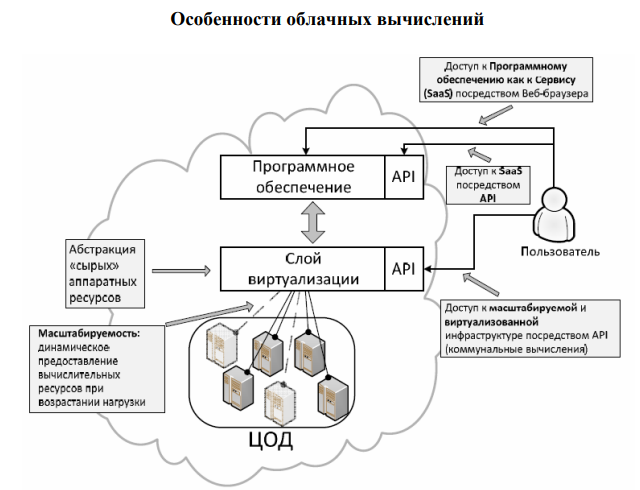
\includegraphics[width=450]{pic15-1}
  \caption{Особенности облачных вычислений}
  \end{center}
  \end{figure}

  Со стороны владельца вычислительных ресурсов облачные вычисления ориентированы на предоставление информационных ресурсов внешним пользователям.

  Со стороны пользователя, облачные вычисления - это получение информационных ресурсов в виде услуги у внешнего поставщика, оплата за которую производится в зависимости от объема потребленных ресурсов согласно установленному тарифу.

  Ключевыми характеристиками облачных вычислений являются масштабируемость и виртуализация.

  Масштабируемость представляет собой возможность динамической настройки информационных ресурсов к изменяющейся нагрузке, например к увеличению или уменьшению количества пользователей, изменению необходимой емкости хранилищ данных или вычислительной мощности.

  Виртуализация в основном используется для обеспечения абстракции и инкапсуляции.

  Абстракция позволяет унифицировать «сырые» вычислительные, коммуникационные ресурсы и хранилища информации в виде пула ресурсов и выстроить унифицированный слой ресурсов, который содержит те же ресурсы, но в абстрагированном виде. Они представляются пользователям и верхним слоям облачных систем как виртуализованные серверы, кластеры серверов, файловые системы и СУБД.

  Инкапсуляция приложений повышает безопасность, управляемость и изолированность.

  Еще одной важной особенностью облачных платформ является интеграция аппаратных ресурсов и системного ПО с приложениями, которые предоставляются конечному пользователю в виде сервисов. 

  Так или иначе, виртуализация позволяет одному компьютеру стать базой для нескольких виртуальных машин, на каждой из которых потенциально может быть запущена совершенно другая операционная система. Преимуществом такого подхода является то, что авария одной виртуальной машины не приводит к аварии любой другой машины. На виртуализированной системе разные серверы могут запускаться на разных виртуальных машинах, поддерживая тем самым модель частичных отказов, характерную для мультикомпьютеров, но при меньшей стоимости и более простом обслуживании. Более того, теперь на одном и том же оборудовании можно запускать несколько разных операционных систем, получая преимущества изолированности виртуальных машин при угрозе хакерских атак и другие преимущества.

  \begin{center}{\bfseries Публичный облачный сервис}
  \end{center}
  Облачная инфраструктура, которой могут пользоваться сразу несколько клиентов, называется публичным облаком. Набор услуг, а также управление аппаратным и программным обеспечением предоставляются поставщиком. Провайдер сдает уже готовые ресурсы в аренду, предоставляя их по требованию с помощью интернета. Публичные облака это ИТ-модель, при которой конфигурацию ресурсов можно менять в процессе работы. Вычислительные системы, инструменты и инфраструктура используются несколькими компаниями. 

  Облако базируется на таких сервисах как IaaS, PaaS, SaaS (инфраструктура, платформа и программное обеспечение как услуга). Распределение ресурсов происходит в соответствии с потребностями заказчиков. Публичное облако может находиться в собственности поставщика услуг. Виртуальные устройства не отличаются функциональностью от физического сервера. 

  Виртуальные машины, которые используют арендаторы, размещены в дата-центре, и обслуживаются персоналом компании-поставщика. Для создания и работы публичного облака необходима совокупность программного и аппаратного обеспечения. Виртуализацию ресурсов, автоматизацию опции самообслуживания, административный контроль обеспечивает применение набора технологий. Публичным этот вид облака называется потому, что его услуги получают несколько заказчиков. Это могут быть как отдельные, обычные пользователи, так и целые организации.

  \begin{center}{\bfseries Приватный облачный сервис}
  \end{center}

  Приватные облака строятся в пределах одной организации или её филиальное сети и служат для осуществления облачных вычислений внутри организации. Любая облачная инфраструктура имеет базовые вычислительные ресурсы, такие как ЦП и хранилище, которые предоставляются по запросу через портал самообслуживания. В частном облаке все ресурсы изолированы и контролируются одной организации. Частное облако также называют внутренним или корпоративным облаком.

  До того, как компания Amazon представила облачные сервисы, большинство компаний приобретали и обслуживали аппаратные средства, такие как серверы, устройства хранения данных и сетевые устройства. Они хранили это оборудование в своих внутренних локальных центрах обработки данных и в центрах совместного размещения для поддержки своих ИТ-операций. После того как мы запустили Amazon Web Services (AWS), компании попытались воспроизвести модель облачных вычислений на своей внутренней инфраструктуре. Термин частное облако был введен, чтобы провести различие между этими внутренними облачными средами и сторонними общедоступными облачными сервисами.

  \newpage 
  \chapter{Тема 16 ОС мобильных устройств}

  \begin{center}{\bfseries Виды мобильных ОС}
  \end{center}

  \begin{opr}
    Мобильная операционная система (мобильная ОС) — операционная система для смартфонов, планшетов, КПК или других мобильных устройств.
  \end{opr}

  Хотя ноутбуки и можно отнести к мобильным устройствам, однако операционные системы, обычно используемые на них, мобильными не считаются, так как изначально разрабатывались для крупных стационарных настольных компьютеров, которые традиционно не нуждались в специальных «мобильных» функциях. Это различие размыто в некоторых новых операционных системах, представляющих гибрид того и другого.

  Мобильные операционные системы сочетают в себе функциональность Операционных Систем для ПК с функциями для мобильных и карманных устройств: сенсорный экран, сотовая связь, Bluetooth, Wi-Fi, GPS-навигация, камера, видеокамера, распознавание речи, диктофон, музыкальный плеер, NFC и инфракрасное дистанционное управление.

  Портативные устройства мобильной связи (например, смартфоны) содержат две операционные системы. Основную программную платформу взаимодействия с пользователем дополняет вторая, низкоуровневая проприетарная операционная система реального времени, обслуживающая радиооборудование. Исследования показали, что такие низкоуровневые операционные системы уязвимы перед вредоносными базовыми станциями, способными получить контроль над мобильным устройством.

  \begin{example}
    Современные операционные системы для мобильных устройств: Android, Kai OS, Lineage OS, Fire OS, Flyme OS, iOS, Sailfish OS, Tizen, MIUI, Remix OS, Fuchsia Os, Аврора.
  \end{example}

  \begin{example}
    Устаревшие, ныне не поддерживаемые программные платформы: Windows 10 Mobile, Symbian, Windows Mobile, Palm OS, webOS, Maemo, MeeGo, LiMo, BlackBerry OS, Firefox OS, Bada OS, Java OS, Яндекс.Кит.
  \end{example}

  \begin{center}{\bfseries Встраиваемые ОС}
  \end{center}

  \begin{opr}
    Встраиваемая система — специализированная микропроцессорная система управления, контроля и мониторинга, концепция разработки которой заключается в том, что такая система будет работать, будучи встроенной непосредственно в устройство, которым она управляет.
  \end{opr}

  \begin{utv}
    В связи с тем, что система управления будет размещаться внутри более сложного устройства, при её разработке ключевую роль играют следующие факторы:
    \begin{enumerate}
      \item Минимальное собственное энергопотребление (возможно, автономное питание);
      \item Минимальные собственные габариты и вес;
      \item Собственная защита (корпус) минимальна и обеспечивается прочностью и жёсткостью конструкции, и применёнными элементами;
      \item Функции отвода тепла (охлаждения) обеспечивают минимум требований тепловых режимов. Если плотность теплового потока (тепловой поток, проходящий через единицу поверхности) не превышает 0,5 мВт/см², перегрев поверхности устройства относительно окружающей среды не превысит 0,5 °C, такая аппаратура считается не теплонагруженной и не требует специальных схем охлаждения.
      \item Микропроцессор и системная логика, а также ключевые микросхемы по возможности совмещены на одном кристалле;
      \item Специальные военно-космические требования по радиационной и электромагнитной стойкости, работоспособность в вакууме, гарантированное время наработки, срок доступности решения на рынке и т. д.
    \end{enumerate}
  \end{utv}

  \begin{utv}
    Областью применения встроенных систем являются:
    \begin{enumerate}
      \item Cредства автоматического регулирования и управления технологическими процессами, например, авионика, контроль доступа;
      \item Cтанки с ЧПУ;
      \item Банкоматы, платёжные терминалы;
      \item Телекоммуникационное оборудование.
    \end{enumerate}
  \end{utv}

  Некоторые встроенные системы находят массовое применение, например, устройства RFID. Встроенные системы являются привлекательной целью для создателей вредоносного кода из-за своей распространённости и относительной беззащитности. Постепенно злоумышленники пытаются создать вредоносный код для встроенных систем (например, RFID-вирус, Cabir). Этот процесс пока затрудняется разнородностью встроенных устройств, отсутствием доминирующего ПО и ограниченной функциональностью некоторых видов устройств. С другой стороны, задача антивирусных компаний и исследователей компьютерной безопасности осложнена теми же обстоятельствами, а также маломощностью встроенных систем, зачастую не позволяющей пользоваться распространённым антивирусным ПО.

  Центральным процессорным устройством для встраиваемой системы могут служить очень многие из современных микропроцессоров и микроконтроллеров. Конкретный вид определяется при проектировании, исходя из целей и задач, выполняемых встраиваемой системой.

  \begin{center}{\bfseries Интернет вещей}
  \end{center}

  \begin{opr}
    Интернет вещей — концепция сети передачи данных между физическими объектами («вещами»), оснащёнными встроенными средствами и технологиями для взаимодействия друг с другом или с внешней средой. Предполагается, что организация таких сетей способна перестроить экономические и общественные процессы, исключить из части действий и операций необходимость участия человека.
  \end{opr}

  Концепция сформулирована в 1999 году как осмысление перспектив широкого применения средств радиочастотной идентификации для взаимодействия физических предметов между собой и с внешним окружением. Наполнение концепции многообразным технологическим содержанием и внедрение практических решений для её реализации начиная с 2010-х годов считается устойчивой тенденцией в информационных технологиях, прежде всего, благодаря повсеместному распространению беспроводных сетей, появлению облачных вычислений, развитию технологий межмашинного взаимодействия, началу активного перехода на IPv6[4] и освоению программно-определяемых сетей.

  \begin{center}{\bfseries Средства идентификации}
  \end{center} 

  Задействование в «интернете вещей» предметов физического мира, не обязательно оснащённых средствами подключения к сетям передачи данных, требует применения технологий идентификации этих предметов («вещей»). Хотя толчком для появления концепции стала технология RFID, но в качестве таких технологий могут использоваться все средства, применяемые для автоматической идентификации: оптически распознаваемые идентификаторы (штрихкоды, Data Matrix, QR-коды), средства определения местонахождения в режиме реального времени. При всеобъемлющем распространении «интернета вещей» принципиально обеспечить уникальность идентификаторов объектов, что, в свою очередь, требует стандартизации.

  Для объектов, непосредственно подключённых к интернет-сетям, традиционный идентификатор — MAC-адрес сетевого адаптера, позволяющий идентифицировать устройство на канальном уровне, при этом диапазон доступных адресов практически неисчерпаем (248 адресов в пространстве MAC-48), а использование идентификатора канального уровня не слишком удобно для приложений. Более широкие возможности по идентификации для таких устройств даёт протокол IPv6, обеспечивающий уникальными адресами сетевого уровня не менее 300 млн устройств на одного жителя Земли.

  \begin{center}{\bfseries Средства измерения}
  \end{center}

  Особую роль в интернете вещей играют средства измерения, обеспечивающие преобразование сведений о внешней среде в машиночитаемые данные, и тем самым наполняющие вычислительную среду значимой информацией. Используется широкий класс средств измерения, от элементарных датчиков (например, температуры, давления, освещённости), приборов учёта потребления (таких, как интеллектуальные счётчики) до сложных интегрированных измерительных систем. В рамках концепции «интернета вещей» принципиально объединение средств измерения в сети (такие, как беспроводные датчиковые сети, измерительные комплексы), за счёт чего возможно построение систем межмашинного взаимодействия.

  Как особая практическая проблема внедрения «интернета вещей» отмечается необходимость обеспечения максимальной автономности средств измерения, прежде всего, проблема энергоснабжения датчиков. Нахождение эффективных решений, обеспечивающих автономное питание сенсоров (использование фотоэлементов, преобразование энергии вибрации, воздушных потоков, использование беспроводной передачи электричества), позволяет масштабировать сенсорные сети без повышения затрат на обслуживание (в виде смены батареек или подзарядки аккумуляторов датчиков).

  \begin{center}{\bfseries Средства передачи данных}
  \end{center}

  Спектр возможных технологий передачи данных охватывает все возможные средства беспроводных и проводных сетей.

  Для беспроводной передачи данных особо важную роль в построении «интернета вещей» играют такие качества, как эффективность в условиях низких скоростей, отказоустойчивость, адаптивность, возможность самоорганизации. Основной интерес в этом качестве представляет стандарт IEEE 802.15.4, определяющий физический слой и управление доступом для организации энергоэффективных персональных сетей, и являющийся основой для таких протоколов, как ZigBee, WirelessHart, MiWi, 6LoWPAN, LPWAN.

  Среди проводных технологий важную роль в проникновении «интернета вещей» играют решения PLC — технологии построения сетей передачи данных по линиям электропередачи, так как во многих приложениях присутствует доступ к электросетям (например, торговые автоматы, банкоматы, интеллектуальные счётчики, контроллеры освещения изначально подключены к сети электроснабжения). 6LoWPAN, реализующий слой IPv6 как над IEEE 802.15.4, так и над PLC, будучи открытым протоколом, стандартизуемым IETF, отмечается как особо важный для развития «интернета вещей».

  